%---------------------------------------------------
%----- Calculation of the Root Hashes
%---------------------------------------------------
\subsection{Calculation of the Root Hashes}
Every root hash of a document $R_{\texttt{doc-root}}$ is stored in the
\textit{AnchorRepository} smart contract. The document root hash is calculated from three different Merkle trees (see Fig. \ref{fig:root-hash}). 
\subsubsection{Merkle Tree of Fields}
A Merkle tree is a way to calculate a unique hash from a set of items. We formally define a Merkle tree function $\mathcal{M}$ to calculate a root hash $R \in \mathbb{B}_{32}$ of document fields $F$. The implementation of the Merkle tree function is introduced in Sec. \ref{sec:precise_proofs}.
 \begin{eqnarray}
 R & = &\mathcal{M}(F_{[0]},...,F_{[n]}) \\
 R & \in & \mathbb{B}_{32}
\end{eqnarray}
\newline
\subsubsection{Model Merkle tree}
As a first step, we calculate the Merkle tree of the schema fields $S$ and the core document fields $C$ of a document $d$.\\
As a second step, we flatten and combine all leaves from each tree.\\ 
Finally, we calculate the Model Merkle Root\\\\
\textbf{Model Root} The Merkle root of the flattened document schema and the core document data, formally $R_{{\texttt{model}}}$ 
\newline
\begin{equation}
    d_M = (d_S + d_C)
\end{equation}
\begin{equation}
    R_{{\texttt{model}}} = \mathcal{M}(d_M)
\end{equation}
\newline
 \subsubsection{Basic and ZK Model trees}
\textbf{Basic Model} The Merkle tree of the flattened document schema and the core document data, formally $R_{{\texttt{basic-model}}}$
\newline
\begin{equation}
    R_{{\texttt{basic-model}}} = \mathcal{M}(d_{MB})
\end{equation}
\newline
The Basic Model tree has the following properties:
\begin{itemize}  
\item Leaf Hashing function keccak-sha3 (add ref) of 256 bits
\item Node Hashing function blake2b (add ref) of 256 bits
\item Sorted Hashes
\end{itemize}
\newline
\textbf{ZK Model} The Merkle tree of the flattened document schema and the core document data ready for Zero Knowledge proving, formally $R_{{\texttt{zk-model}}}$
\newline
\begin{equation}
    R_{{\texttt{zk-model}}} = \mathcal{M}(d_{MZ})
\end{equation}
\newline
The ZK Model tree has the following properties:
\begin{itemize}  
\item Leaf Hashing function keccak-sha3 of 256 bits
\item Node Hashing function pedersen (add ref) of 256 bits
\item Ordered (Left-Right) Hashes
\item Fixed size of 20 levels
\end{itemize}
 \subsubsection{Signing Root}
The $R_{\texttt{signing}}$ is calculated from the blake2b-256 hash of the concatenated $R_\texttt{basic-model}$ and $R_{\texttt{zk-model}}$
\newline
\begin{equation}
R_{\texttt{signing}} = \texttt{blake2b}(R_\texttt{basic-model}\| R_{\texttt{zk-model}})
\end{equation}\\
We formally define a helper function for calculating the $R_{\texttt{signing}}$ 
\begin{eqnarray}
R_{\texttt{signing}}& =&\mathsf{calculateSigningRoot}(d) \\
\mathsf{calculateSigningRoot}(d)& =& \texttt{blake2b}(\mathcal{M}(d_{MB})\| \mathcal{M}(d_{MZ}))
\end{eqnarray}
 \subsubsection{Signatures Root}
 A Merkle root of the collaborator signature must be part of the document root hash $R_{\texttt{doc-root}}$. The signatures are relevant for the document consensus, explained in the following chapters. \\\\
\textbf{Signature Root} A signature root hash defines the Merkle root of all signatures $d_{\texttt{signatures}}$, formally $R_{\texttt{signatures}}$:
\newline
\begin{equation}
R_{\texttt{signatures}} = \mathcal{M}(d_{\texttt{signatures}})\\
\end{equation}
 \subsubsection{Document Root}
The final  document root hash $R_{\texttt{doc-root}}$ of the entire document $d$ is defined as the blake2b hash of the concatenated signing root hash $R_{\texttt{signing}}$ and signature root hash $R_{\texttt{signatures}}$ 
\newline
 \begin{equation}
R_{\texttt{doc-root}} =  \texttt{blake2b}(R_{\texttt{signing}}\|R_{\texttt{signatures}})
\end{equation}\\
A tree of the  $R_{\texttt{doc-root}}$ calculation. (see Fig. \ref{fig:root-hash})

%TODO (Manuel): Why sometimes R and D?

%All information related to the document is stored in a structured protobuf message called CoreDocument, \mathsf{CD}, along with a document-specific message, Data, \mathsf{D} such as an Invoice or PurchaseOrder. Both messages are serialized with precise proofs into \\mathsf{CD} 

\begin{figure}[thpb]
\centering
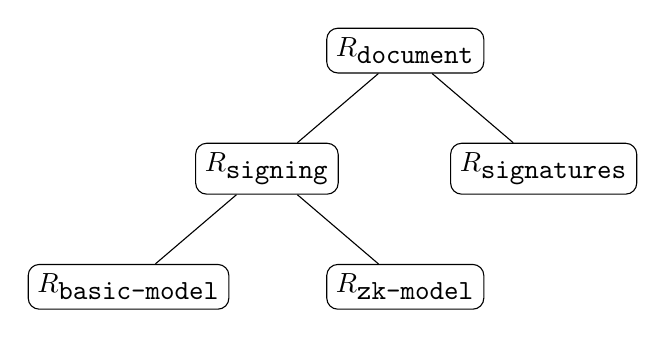
\begin{tikzpicture}[sibling distance=10em,
  every node/.style = {shape=rectangle, rounded corners,
    draw, align=center, %top color=white, bottom color=gray!20
    }]]
  \node {$R_{{\texttt{document}}}$}
    child { node {$R_{{\texttt{signing}}}$}  child { node {$R_{{\texttt{basic-model}}}$}  
    } child { node {$R_{{\texttt{zk-model}}}$} 
    } }
    child { node {$R_{{\texttt{signatures}}}$}};
\end{tikzpicture}
\caption{Calculation of the last layers of the document merkle tree. The leafs are the roots of merkle trees from the different document parts }\label{fig:root-hash}
\end{figure}
We can define a second help function called $\mathsf{calculateDocumentRoot}(d)$ for calculating the entire $R_{\texttt{doc-root}}$. 
\begin{eqnarray}
R_{\texttt{doc-root}}& =&\mathsf{calculateDocumentRoot}(d) \\
\mathsf{calculateDocumentRoot}(d)& = & \texttt{blake2b}( \mathsf{R_{\texttt{signing}}}\| \mathcal{M}_{\texttt{tree}}(d_S))
\end{eqnarray}